\chapter{Wstęp}
\label{cha:wstep}

Laboratorium pojazdów autonomicznych AGH--Delphi ma za zadanie zbudowanie pojazdu autonomicznego na bazie udostępnionego pojazdu elektrycznego (zob. zdjęcie \ref{fig:electric_vehicle}). Podczas prac konieczne jest zapewnienie bezpieczeństwa podczas testowania algorytmów sterowania. Algorytmy takie mogą nie działać poprawnie, w~związku z~czym w~trakcie testów może zajść potrzeba awaryjnego przerwania jazdy samochodu.

\begin{figure}[h]
	\centering
	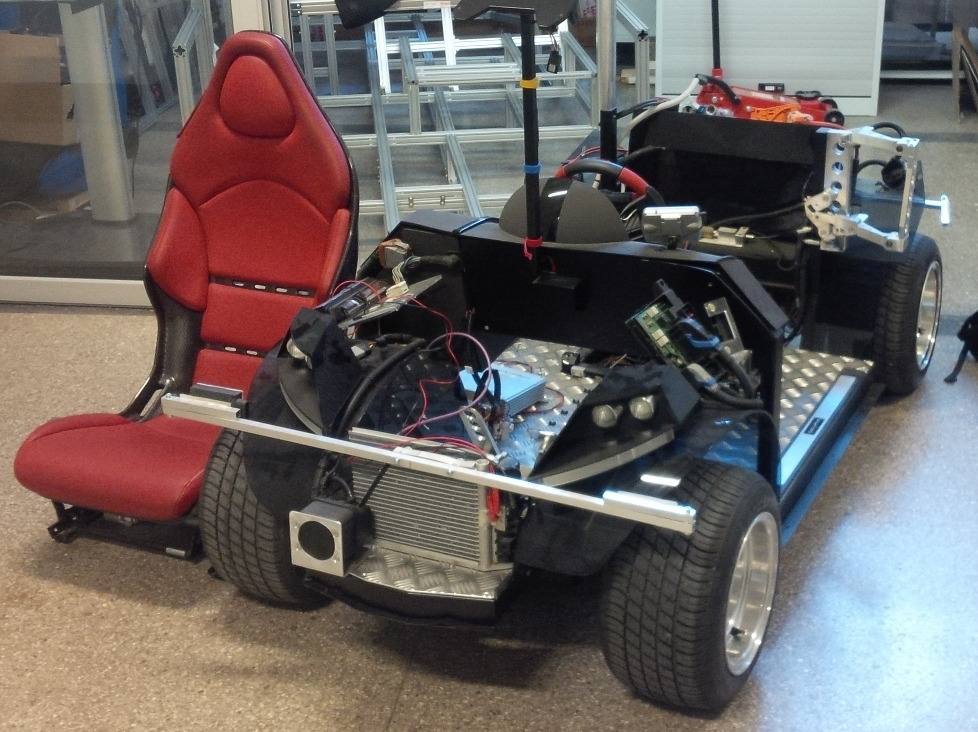
\includegraphics[scale=0.4]{pics/electric_vehicle_scaled.jpg}
	\caption{\label{fig:electric_vehicle}Samochód elektryczny udostępniony przez firmę Delphi (zdjęcie: P. Banaszkiewicz).}
\end{figure}

Awaryjne przerwanie jazdy samochodu powinno odbyć się poprzez wyłączenie zasilania silnika samochodu. O ile jest to możliwe, należy uniknąć odłączenia zasilania reszty samochodu (np. układu kierowniczego lub komputera pokładowego).

%---------------------------------------------------------------------------

\section{Cele projektu}
\label{sec:cele_projektu}

System ESAV (ang. \textit{Emergency Stop Autonomous Vehicle} – zdalny wyłącznik bezpieczeństwa dla samochodu autonomicznego) powinien charakteryzować się następującymi właściwościami:

\begin{itemize}
\item Możliwość natychmiastowego zatrzymania pojazdu na polecenie operatora.
\item Natychmiastowe zatrzymanie pojazdu w przypadku utraty zasilania systemu ESAV.
\item Natychmiastowe zatrzymanie pojazdu w przypadku przerwania transmisji pomiędzy modułami systemu ESAV.
\item Natychmiastowe zatrzymanie pojazdu w przypadku zakłóceń pracy systemu ESAV (na przykład w wyniku błędów transmisji).
\item Możliwość poruszania się pojazdu tylko jeśli system ESAV jest zasilany.
\item Możliwość poruszania się pojazdu tylko w przypadku rozpoczęcia prawidłowej transmisji danych \item pomiędzy modułami systemu ESAV.
\item Możliwość wyświetlenia aktualnego stanu systemu ESAV.
\end{itemize}

W niniejszym opisie projektu używane będą następujące pojęcia skrótowe:
\begin{itemize}
\item \textbf{moduł A}: bazowy moduł systemu ESAV; to z niego korzysta operator aby wyłączyć zasilanie silnika w samochodzie,
\item \textbf{moduł B}: moduł montowany w samochodzie, który odpowiedzialny jest za wyłączenie zasilania silnika,
\item \textbf{tryb awaryjny}: tryb modułu B w którym następuje odłączenie zasilania silnika samochodu.
\end{itemize}

Zasilanie obydwu modułów powinno być całkowicie niezależne od zasilania pojazdu, a wymianę akumulatorów łatwa. Ponadto obydwa moduły muszą monitorować i pokazywać poziom naładowania swoich akumulatorów.

Po wyłączeniu pojazdu przez system ESAV układ musi zostać przywrócony do pracy poprzez zresetowanie.

System ESAV powinien być systemem bezobsługowym: raz skonfigurowany ma poprawnie pracować bez ingerencji użytkownika. Budowa systemu powinna umożliwiać innym osobom kontynuowanie prac nad nim. W tym celu jego oprogramowanie powinno być otwarto-źródłowe, a sprzęt wymienialny.

%---------------------------------------------------------------------------

\section{Wymagania funkcjonalne}
\label{sec:wymagania_funkcjonalne}

Na podstawie opisu z rozdziału \ref{sec:cele_projektu} wyznaczono poniższe cele funkcjonalne systemu ESAV:

\begin{enumerate}[label=\thesection.\arabic{*}.,leftmargin=4em]
\item \label{wym_fun1} Moduł B przy braku zasilania ma odcinać zasilanie silnika samochodu.
\item \label{wym_fun2} Po włączeniu moduł B ma oczekiwać na dane aktywujące jego pracę, które ma otrzymać od modułu A. Stan modułu B sygnalizowany jest migającą czerwoną diodą.
\item \label{wym_fun3} Dopóki moduł B nie odbierze danych aktywujących, pojazd nie może się poruszać.
\item \label{wym_fun4} Po odebraniu danych aktywujących, moduł B powinien umożliwić jazdę samochodu. Stan modułu B sygnalizowany jest świecącą zieloną diodą.
\item \label{wym_fun5} Jeżeli podczas działania moduł B przestanie odbierać transmisję, musi on przejść w tryb awaryjny. Stan modułu sygnalizowany jest ciągle świecącą się czerwoną diodą.
\item \label{wym_fun6} Po naciśnięciu przycisku wyłączenia awaryjnego w module A przez operatora, moduł B musi przejść w tryb awaryjny. Stan modułu sygnalizowany jest ciągle świecącą się czerwoną diodą.
\item \label{wym_fun7} Po zresetowaniu modułu B poprzez naciśnięcie przycisku „Reset”, moduł B powraca z trybu awaryjnego do stanu oczekiwania na dane aktywujące. Stan modułu sygnalizowany jest migającą czerwoną diodą.
\item \label{wym_fun8} Po wyłączeniu zasilania modułu B musi nastąpić odłączenie zasilania silnika samochodu.
\item \label{wym_fun9} Bateria (akumulator) modułu B może być ładowana w trakcie ładowania akumulatorów pojazdu.
\end{enumerate}

%---------------------------------------------------------------------------

\section{Wymagania użytkowe}
\label{sec:wymagania_wydajnosciowe}

Na podstawie opisu z rozdziału \ref{sec:cele_projektu} wyznaczono poniższe cele zasięgu, czasu oraz szybkości działania systemu ESAV:

\begin{enumerate}[label=\thesection.\arabic{*}.,leftmargin=4em]
\item \label{wym_uzyt1} System ESAV musi pracować bez konieczności wymiany bądź ładowania baterii (akumulatorów) przez minimum 5 godzin.
\item \label{wym_uzyt2} System ESAV musi być w stanie co 1 sekundę odbierać i dekodować dane, a następnie je wysyłać.
\item \label{wym_uzyt3} System ESAV musi pracować poprawnie na dystansie 100 metrów w otwartej przestrzeni.
\item \label{wym_uzyt4} System ESAV musi pracować poprawnie w pomieszczeniach.
\end{enumerate}

%---------------------------------------------------------------------------

\section{Wymagania współdziałania}
\label{sec:wymagania_wspoldzialania}

Na podstawie opisu z rozdziału \ref{sec:cele_projektu} wyznaczono poniższe cele integracji systemu ESAV z innymi urządzeniami:

\begin{enumerate}[label=\thesection.\arabic{*}.,leftmargin=4em]
\item \label{wym_wsp1} Moduł B musi poprawnie wyłączać silnik samochodu.
\item \label{wym_wsp2} Moduł B powinien mieć układ ładujący podłączony do systemu elektrycznego pojazdu.
\end{enumerate}

%---------------------------------------------------------------------------

\section{Wymagania bezpieczeństwa}
\label{sec:wymagania_bezpieczenstwa}

Na podstawie opisu z rozdziału \ref{sec:cele_projektu} wyznaczono poniższe wymagania bezpieczeństwa przy korzystaniu z systemu ESAV:
\begin{enumerate}[label=\thesection.\arabic{*}.,leftmargin=4em]
\item \label{wym_bezp1} Moduł B systemu ESAV nie może doprowadzić do porażenia użytkownika prądem.
\item \label{wym_bezp2} Komunikacja pomiędzy modułami powinna zabezpieczać przed atakami powtórzenia poleceń operatora.
\item \label{wym_bezp3} Moduł B systemu ESAV nie może nagrzewać się powyżej temperatury \SI{50}{\celsius}.
\end{enumerate}

%---------------------------------------------------------------------------

\section{Wymagania pochodne}
\label{sec:wymagania_pochodne}

Wymagania, które nie zostały jawnie wspomniane w rozdziałach \ref{sec:wymagania_funkcjonalne}—\ref{sec:wymagania_bezpieczenstwa}, a wynikają albo z opisu projektu (rozdział \ref{sec:cele_projektu}), albo pojawiły się w momencie implementowania projektu, zostały opisane w tym rozdziale.

Moduł B musi:

\begin{enumerate}[label=\thesection.\arabic{*}.,leftmargin=4em]
\item \label{wym_poch1} monitorować poziom naładowania (napięcie) na baterii zasilającej,
\item \label{wym_poch2} sygnalizować włączenie trybu awaryjnego świeceniem czerwonej diody,
\item \label{wym_poch3} sygnalizować oczekiwanie na transmisję miganiem czerwonej diody,
\item \label{wym_poch4} sygnalizować poprawne działanie świeceniem zielonej diody.
\end{enumerate}

Moduł A musi:

\begin{enumerate}[label=\thesection.\arabic{*}.,leftmargin=4em]
\setcounter{enumi}{4}
\item \label{wym_poch5} monitorować poziom naładowania (napięcie) na baterii zasilającej,
\item \label{wym_poch6} sygnalizować wysyłanie informacji miganiem zielonej diody,
\item \label{wym_poch7} mieć małe wymiary (aby możliwe było trzymania go w dłoniach).
\end{enumerate}

Komunikacja między modułami powinna umożliwiać wymianę takich informacji:

\begin{enumerate}[label=\thesection.\arabic{*}.,leftmargin=4em]
\setcounter{enumi}{7}
\item \label{wym_poch8} PING: wymiana danych co około sekundę (do weryfikacji istnienia połączenia),
\item \label{wym_poch9} STOP: do wysłania danych w celu natychmiastowego przejścia modułu B w tryb awaryjny,
\item \label{wym_poch10} DATA: do wymiany danych diagnostycznych (np. napięcia baterii).
\end{enumerate}


%---------------------------------------------------------------------------

\section{Podsumowanie}
\label{sec:wstep_podsumowanie}

Podejście do projektu oparte o listę wymagań (ang. \textit{requirements-driven design} \cite{Hug10} albo \textit{feature-driven development} \cite{Goy08}) umożliwia sprecyzowanie niewielkich wymagań a priori, które pozwalają wykonawcy implementować funkcjonalności pojedyncze i skierowane na konkretne wymagania, a także śledzić spełnienie tych wymagań w formie prostej tabeli (zob. rozdział \ref{sec:zrealizowane_wymagania}).

W tym rozdziale zostały wyszczególnione wymagania według sugerowanego schematu z~\cite{Hug10}, jednakże w przypadku projektów stricte programistycznych schemat ten może wyglądać inaczej.

Skupienie się na wyszczególnieniu wymagań przed rozpoczęciem prac nad projektem znacząco ułatwiło jego tworzenie, m.in. poprzez eliminację luk w opisie funkcjonalnym systemu ESAV.

\begin{figure}[h]
	\centering
	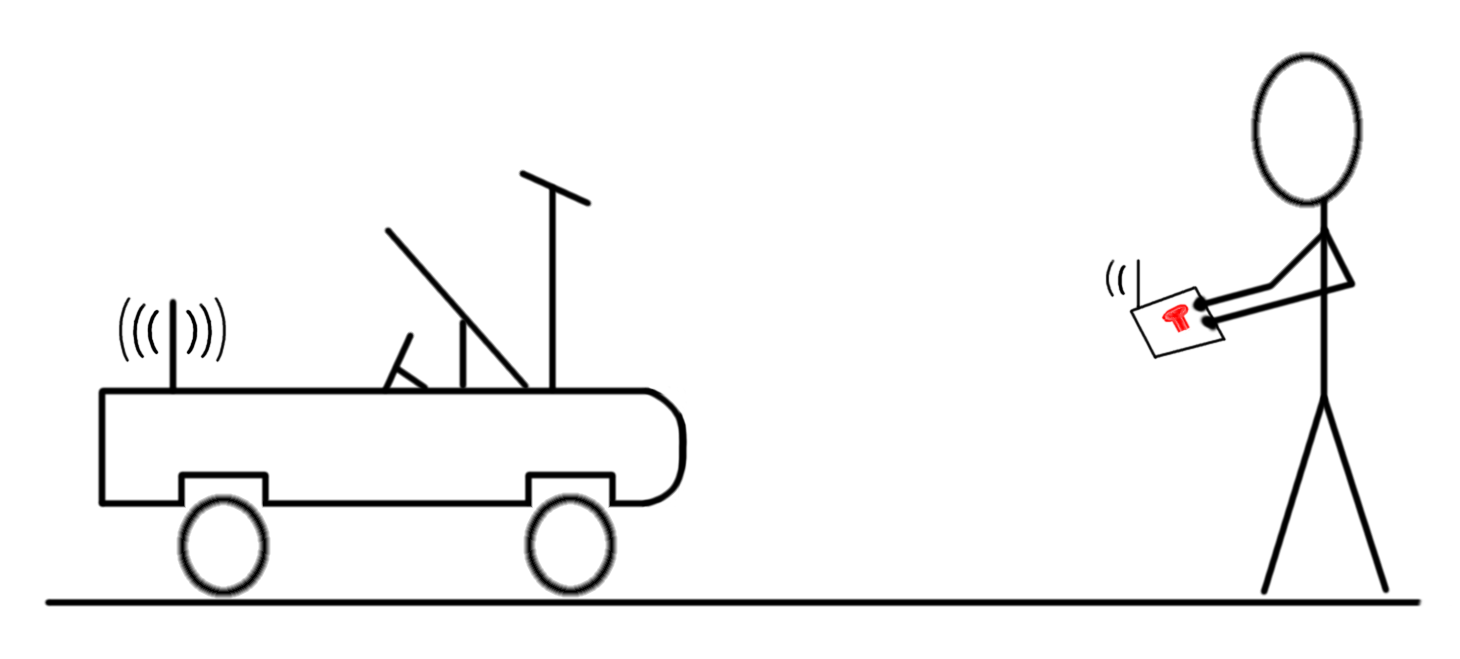
\includegraphics[scale=0.3]{pics/preview_cartoon.png}
	\caption{\label{fig:preview}Rysunek poglądowy systemu w trakcie działania (rysenek: P. Banaszkiewicz).}
\end{figure}
